\documentclass[UTF8,a4paper,zihao=-4,oneside,onecolumn,scheme=chinese,autoindent=true]{ctexbook}
\usepackage{xcolor}
\usepackage{clrscode3e}
\usepackage{float}
\usepackage{tabularx}
\usepackage[hmargin=2.5cm,vmargin=2.5cm]{geometry}
\usepackage{verbatim}
\usepackage{fontspec}


\usepackage{listings}
\definecolor{mygreen}{rgb}{0,0.6,0}
\definecolor{mygray}{rgb}{0.5,0.5,0.5}
\definecolor{mymauve}{rgb}{0.58,0,0.82}
\lstset{ %
    backgroundcolor=\color{white},   % choose the background color
    commentstyle=\color{mygreen}\ttfamily,    % comment style
    keywordstyle=\color{blue}\bfseries\underbar,       % keyword style
    stringstyle=\color{mymauve}\ttfamily,     % string literal style
    % basicstyle=\footnotesize\ttfamily,        % size of fonts used for the code
    basicstyle=\small\ttfamily,        % size of fonts used for the code
    numbers=left,
    numberstyle=\tiny,
    stepnumber=1,
    numbersep=5pt,
    columns=fullflexible,
    breaklines=true,                 % automatic line breaking only at whitespace
    captionpos=b,                    % sets the caption-position to bottom
    tabsize=4,
    escapeinside={\%*}{*)},          % if you want to add LaTeX within your code
    frame=single,
    rulesepcolor=\color{red!20!green!20!blue!20}
    % identifierstyle=\color{red}
}

\lstdefinestyle{Python}{
    language=Python
}
\lstdefinestyle{CPP}{
    language=[11]C++,
    morekeywords={std,vector}
}
% latex + dvipdfmx 编译方式要在 tikz 宏包之前调用 graphicx 宏包并指定 dvipdfmx 选项. 
\usepackage{graphicx}
\usepackage{tikz}

\title{算法导论学习笔记}
\author{Yaohui Li}
\date{\today}

\begin{document}

\maketitle

\tableofcontents

%第一部分
\part{基础知识}

%第一章
\chapter{算法在计算中的作用}
%第1.1节
\section{算法}
\textbf{算法}(algorithm)就是任何良定义的计算过程, 该过程取某个值或值的集合作为\textbf{输入}并产生某个值或值的集合作为\textbf{输出}. 这样算法就是把输入转换成输出的计算步骤的一个序列.

\subsection*{练习}
\begin{enumerate}
    \renewcommand{\labelenumi}{\thesection-\theenumi}
    \item {\textbf{给出现实生活中需要排序的一个例子或者现实生活中需要计算凸壳的例子. }\\需要排序的例子为: 展示排行榜, 微博热搜榜单等. 需要计算凸壳(凸包)的例子: 割平面法求解线性整数规划问题. }
    \item {\textbf{除速度外, 在真实环境中还可能使用哪些其它有关效率的量度? }\\计算步骤的复杂性, 计算过程所需的内存空间大小等. }
    \item {\textbf{选择一种你以前已知的数据结构, 并讨论其优势和局限. }\\以数组为例. 优势: 结构简单, 容易实现. 局限: 删除元素效率低下. }
    \item {\textbf{前面给出的最短路径与旅行商问题有哪些相似之处? 又有哪些不同? }\\相似之处: 都属于图论中的问题, 且优化目标均为最小化总距离. 不同点: 受到的约束不同, 最短路径问题不需要遍历每一个节点. }
    \item {\textbf{提供一个现实生活的问题, 其中只有最佳解才行. 然后提供一个问题, 其中近似最佳的解也足够好. }\\必须找到最佳解的问题: 找到班级中身高最高的同学. 近似最佳的解也足够好的问题: 装机时, 找到一个比总用电功率大的任意一个电源. }
\end{enumerate}

%第1.2节
\section{作为一种技术的算法}
算法的效率主要体现在时间和空间这两个方面, 因为计算机不可能是无限快的, 存储空间也不是免费的.

\subsection*{练习}
\begin{enumerate}
    \renewcommand{\labelenumi}{\thesection-\theenumi}
    \item {\textbf{给出在应用层需要算法内容的应用的一个例子, 并讨论涉及的算法的功能. }\\加载包含大量图片的网页时, 图片的加载顺序问题. 算法应当首先加载用户最先看到的图片. }
    \item {\textbf{假设我们正比较插入排序与归并排序在相同机器上的实现. 对规模为$n$的输入, 插入排序运行$8n^2$步, 而归并排序运行$64n\lg{n}$步. 问对哪些$n$值, 插入排序优于归并排序? }\\若需插入排序优于归并排序, 则需$n$满足不等式: $8n^2 \le 64n\lg{n}$. 解得: $2 \leq n \leq 43$. }
    \item {\textbf{$n$的最小值为何值时, 运行时间为$100n^2$的一个算法在相同机器上快于运行时间为$2^n$的另一个算法? }\\原问题等价于求解满足不等式: $100n^2 \le 2^n$的最小的$n$. 解得: $n \geq 15$. }
\end{enumerate}

%思考题
\section{思考题}
\begin{enumerate}
    \renewcommand{\labelenumi}{\thechapter-\theenumi}
    \item {
          \textbf{(运行时间的比较)假设求解问题的算法需要$f(n)$毫秒, 对下表中的每个函数$f(n)$和时间$t$, 确定可以在时间$t$内求解的问题的最大规模$n$. }\\
          基本的计算思路是求解满足不等式: $f(n) \leq t$的最大的$n$. 求解结果如下表所示:
          \begin{table}[H]
              \centering
              \begin{tabularx}{\textwidth}
                  {*{7}{>{\centering\arraybackslash}X|}>{\centering\arraybackslash}X}
                  \hline
                             & 1秒钟($10^3$毫秒) & 1分钟($6 \times 10^4$毫秒) & 1小时($3.6 \times 10^6$毫秒) & 1天($8.64 \times 10^7$毫秒) & 1月($2.60 \times 10^9$毫秒) & 1年($3.15 \times 10^{10}$毫秒) & 1世纪($3.15 \times 10^{12}$毫秒) \\ \hline
                  $\lg{n}$   & $2^{10^3}$    & $2^{6 \times 10^4}$    & $2^{3.6 \times 10^6}$    & $2^{8.64 \times 10^7}$   & $2^{2.60 \times 10^9}$   & $2^{3.15 \times 10^{10}}$   & $2^{3.15 \times 10^{12}}$    \\ \hline
                  $\sqrt{n}$ & $10^6$        & $3.6\times10^{9}$      & $1.30\times10^{13}$      & $7.65\times10^{15}$      & $6.72\times10^{18}$      & $9.95\times10^{20}$         & $9.95\times10^{24}$          \\ \hline
                  $n$        & $10^3$        & $6 \times 10^4$        & $3.6 \times 10^6$        & $8.64 \times 10^7$       & $2.60 \times 10^9$       & $3.15 \times 10^{10}$       & $3.15 \times 10^{12}$        \\ \hline
                  $n\lg{n}$  & $140$         & $4895$                 & $2.04\times10^{5}$       & $3.94\times10^{6}$       & $9.79\times10^{7}$       & $1.05\times10^{9}$          & $8.67\times10^{7}$           \\ \hline
                  $n^2$      & $31$          & $244$                  & $1897$                   & $9295$                   & $50990$                  & $177482$                    & $1774823$                    \\ \hline
                  $n^3$      & $10$          & $39$                   & $153$                    & $442$                    & $1375$                   & $3158$                      & $14658$                      \\ \hline
                  $2^n$      & $9$           & $15$                   & $21$                     & $26$                     & $31$                     & $34$                        & $41$                         \\ \hline
                  $n!$       & $6$           & $8$                    & $9$                      & $11$                     & $12$                     & $13$                        & $15$                         \\ \hline
              \end{tabularx}
          \end{table}
          }
\end{enumerate}

%第二章
\chapter{算法基础}
%第1节
\section{插入排序}
\subsection*{插入排序}
插入排序的算法描述为:
\begin{codebox}
    \Procname{$\proc{Insertion-Sort}(A)$}
    \li \For $j \gets 2$ \To $\attrib{A}{length}$
    \li \Do
    $\id{key} \gets A[j]$
    \li \Comment Insert $A[j]$ into the sorted sequence
    $A[1 \twodots j-1]$.
    \li $i \gets j-1$
    \li \While $i > 0$ and $A[i] > \id{key}$
    \li \Do
    $A[i+1] \gets A[i]$
    \li $i \gets i-1$
    \End
    \li $A[i+1] \gets \id{key}$
    \End
\end{codebox}

插入排序的C++代码为:
\lstinputlisting[style=CPP]{./codes/insert_sort.cpp}

以数组$A=[5,2,4,6,1,3]$为例, 该数组的初始状态如图\ref{数组A插入排序前的初始状态}所示. 对该数组进行非降序的排列后, 其状态应该如图\ref{数组A插入排序后的终止状态}所示.

\begin{figure}[H]
    \centering
    \begin{minipage}{0.45\textwidth}
        \centering
        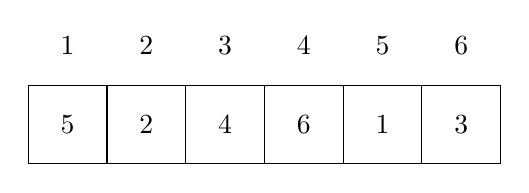
\begin{tikzpicture}
            %绘制数组上方的索引1,2,3,4,5,6
            \foreach \i in {1,2,...,6}{\draw (\i,0)+(-.5,+1.5) node {\i};}
            %绘制数组矩形
            \foreach \i in {0,1,...,5}{\draw (\i,0) rectangle (\i + 1,1);}
            %绘制数组中每个元素值
            \node (A) at (0.5, 0.5) {5};
            \node (B) at (1.5, 0.5) {2};
            \node (C) at (2.5, 0.5) {4};
            \node (D) at (3.5, 0.5) {6};
            \node (E) at (4.5, 0.5) {1};
            \node (F) at (5.5, 0.5) {3};
        \end{tikzpicture}
        \caption{排序前}\label{数组A插入排序前的初始状态}
    \end{minipage}
    % \qquad
    \begin{minipage}{0.45\textwidth}
        \centering
        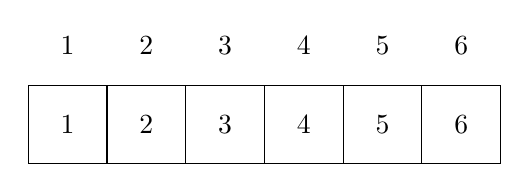
\begin{tikzpicture}
            %绘制数组上方的索引1,2,3,4,5,6
            \foreach \i in {1,2,...,6}{\draw (\i,0)+(-.5,+1.5) node {\i};}
            %绘制数组矩形
            \foreach \i in {0,1,...,5}{\draw (\i,0) rectangle (\i + 1,1);}
            %绘制数组中每个元素值
            \node (A) at (0.5, 0.5) {1};
            \node (B) at (1.5, 0.5) {2};
            \node (C) at (2.5, 0.5) {3};
            \node (D) at (3.5, 0.5) {4};
            \node (E) at (4.5, 0.5) {5};
            \node (F) at (5.5, 0.5) {6};
        \end{tikzpicture}
        \caption{排序后}\label{数组A插入排序后的终止状态}
    \end{minipage}
\end{figure}

采用插入排序的算法流程可以用图\ref{数组$A$的插入排序流程}进行表示:

\begin{figure}[H]
    \centering
    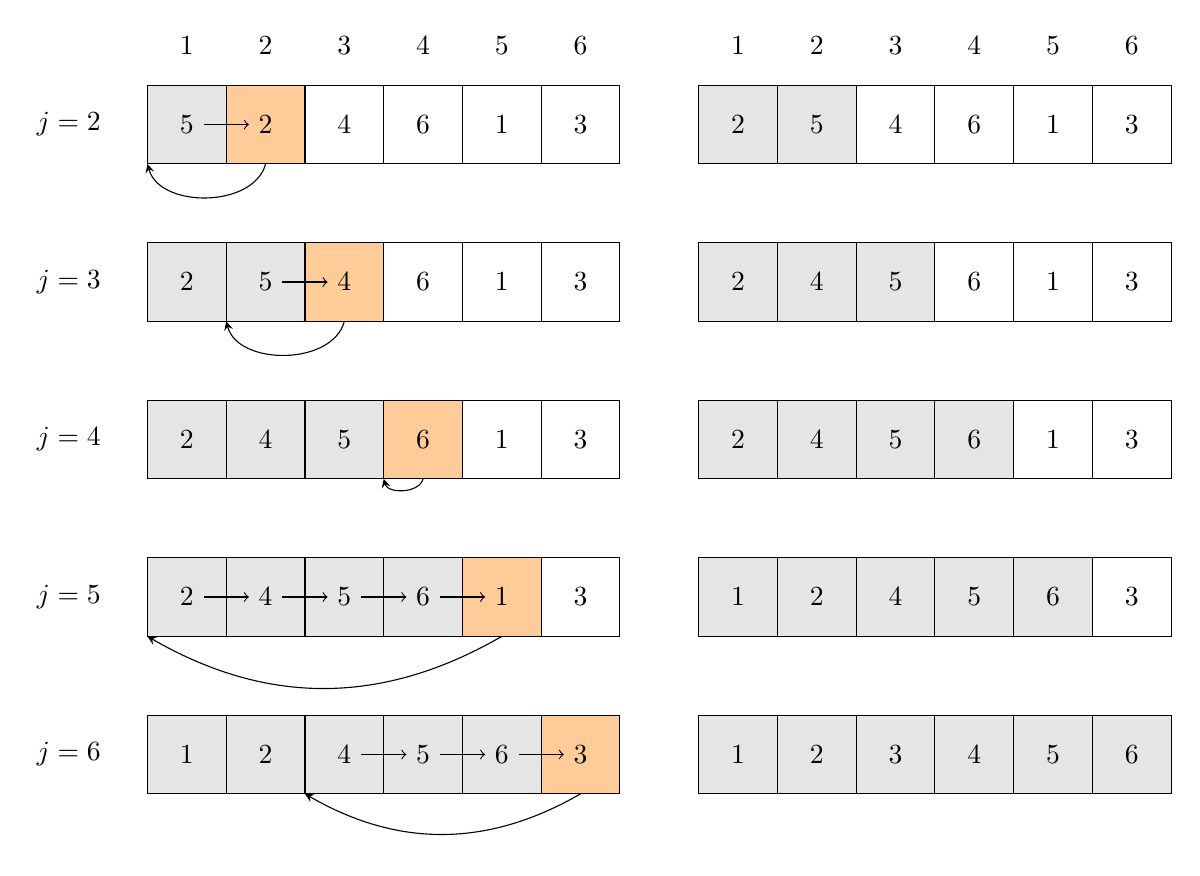
\begin{tikzpicture}
        %绘制数组上方的索引1,2,3,4,5,6
        \foreach \i in {1,2,...,6}{\draw (\i,0)+(-.5,+1.5) node {\i};}
        \foreach \i in {1,2,...,6}{\draw (\i,0)+(6.5,+1.5) node {\i};}
        %j=2
        \node (j_2) at (-1,+.5) {$j=2$};
        %绘制数组矩形
        \draw[fill=black!10] (0,0) rectangle (1,1);
        \draw[fill=orange!40] (1,0) rectangle (2,1);
        \draw (2,0) rectangle (3,1);
        \draw (3,0) rectangle (4,1);
        \draw (4,0) rectangle (5,1);
        \draw (5,0) rectangle (6,1);

        \draw[fill=black!10] (7,0) rectangle (8,1);
        \draw[fill=black!10] (8,0) rectangle (9,1);
        \draw (9,0) rectangle (10,1);
        \draw (10,0) rectangle (11,1);
        \draw (11,0) rectangle (12,1);
        \draw (12,0) rectangle (13,1);
        %绘制数组中每个元素值
        \node (A) at (0.5, 0.5) {5};
        \node (B) at (1.5, 0.5) {2};
        \node (C) at (2.5, 0.5) {4};
        \node (D) at (3.5, 0.5) {6};
        \node (E) at (4.5, 0.5) {1};
        \node (F) at (5.5, 0.5) {3};

        \node (A_) at (7.5, 0.5) {2};
        \node (B_) at (8.5, 0.5) {5};
        \node (C_) at (9.5, 0.5) {4};
        \node (D_) at (10.5, 0.5) {6};
        \node (E_) at (11.5, 0.5) {1};
        \node (F_) at (12.5, 0.5) {3};
        %绘制箭头
        \draw [-stealth] (1.5,0) to[bend left=75] (0,0);
        \draw [->] (A.east) -- (B.west);

        %j=3
        \node (j_3) at (-1,-1.5) {$j=3$};
        %绘制数组矩形
        \draw[fill=black!10] (0,-2) rectangle (1,-1);
        \draw[fill=black!10] (1,-2) rectangle (2,-1);
        \draw[fill=orange!40] (2,-2) rectangle (3,-1);
        \draw (3,-2) rectangle (4,-1);
        \draw (4,-2) rectangle (5,-1);
        \draw (5,-2) rectangle (6,-1);

        \draw[fill=black!10] (7,-2) rectangle (8,-1);
        \draw[fill=black!10] (8,-2) rectangle (9,-1);
        \draw[fill=black!10] (9,-2) rectangle (10,-1);
        \draw (10,-2) rectangle (11,-1);
        \draw (11,-2) rectangle (12,-1);
        \draw (12,-2) rectangle (13,-1);
        %绘制数组中每个元素值
        \node (A) at (0.5, -1.5) {2};
        \node (B) at (1.5, -1.5) {5};
        \node (C) at (2.5, -1.5) {4};
        \node (D) at (3.5, -1.5) {6};
        \node (E) at (4.5, -1.5) {1};
        \node (F) at (5.5, -1.5) {3};

        \node (A_) at (7.5, -1.5) {2};
        \node (B_) at (8.5, -1.5) {4};
        \node (C_) at (9.5, -1.5) {5};
        \node (D_) at (10.5, -1.5) {6};
        \node (E_) at (11.5, -1.5) {1};
        \node (F_) at (12.5, -1.5) {3};
        %绘制箭头
        \draw [-stealth] (2.5,-2) to[bend left=75] (1,-2);
        \draw [->] (B.east) -- (C.west);

        %j=4
        \node (j_4) at (-1,-3.5) {$j=4$};
        %绘制数组矩形
        \draw[fill=black!10] (0,-4) rectangle (1,-3);
        \draw[fill=black!10] (1,-4) rectangle (2,-3);
        \draw[fill=black!10] (2,-4) rectangle (3,-3);
        \draw[fill=orange!40] (3,-4) rectangle (4,-3);
        \draw (4,-4) rectangle (5,-3);
        \draw (5,-4) rectangle (6,-3);

        \draw[fill=black!10] (7,-4) rectangle (8,-3);
        \draw[fill=black!10] (8,-4) rectangle (9,-3);
        \draw[fill=black!10] (9,-4) rectangle (10,-3);
        \draw[fill=black!10] (10,-4) rectangle (11,-3);
        \draw (11,-4) rectangle (12,-3);
        \draw (12,-4) rectangle (13,-3);
        %绘制数组中每个元素值
        \node (A) at (0.5, -3.5) {2};
        \node (B) at (1.5, -3.5) {4};
        \node (C) at (2.5, -3.5) {5};
        \node (D) at (3.5, -3.5) {6};
        \node (E) at (4.5, -3.5) {1};
        \node (F) at (5.5, -3.5) {3};

        \node (A_) at (7.5, -3.5) {2};
        \node (B_) at (8.5, -3.5) {4};
        \node (C_) at (9.5, -3.5) {5};
        \node (D_) at (10.5, -3.5) {6};
        \node (E_) at (11.5, -3.5) {1};
        \node (F_) at (12.5, -3.5) {3};
        %绘制箭头
        \draw [-stealth] (3.5,-4) to[bend left=75] (3,-4);

        %j=5
        \node (j_5) at (-1,-5.5) {$j=5$};
        %绘制数组矩形
        \draw[fill=black!10] (0,-6) rectangle (1,-5);
        \draw[fill=black!10] (1,-6) rectangle (2,-5);
        \draw[fill=black!10] (2,-6) rectangle (3,-5);
        \draw[fill=black!10] (3,-6) rectangle (4,-5);
        \draw[fill=orange!40] (4,-6) rectangle (5,-5);
        \draw (5,-6) rectangle (6,-5);

        \draw[fill=black!10] (7,-6) rectangle (8,-5);
        \draw[fill=black!10] (8,-6) rectangle (9,-5);
        \draw[fill=black!10] (9,-6) rectangle (10,-5);
        \draw[fill=black!10] (10,-6) rectangle (11,-5);
        \draw[fill=black!10] (11,-6) rectangle (12,-5);
        \draw (12,-6) rectangle (13,-5);
        %绘制数组中每个元素值
        \node (A) at (0.5, -5.5) {2};
        \node (B) at (1.5, -5.5) {4};
        \node (C) at (2.5, -5.5) {5};
        \node (D) at (3.5, -5.5) {6};
        \node (E) at (4.5, -5.5) {1};
        \node (F) at (5.5, -5.5) {3};

        \node (A_) at (7.5, -5.5) {1};
        \node (B_) at (8.5, -5.5) {2};
        \node (C_) at (9.5, -5.5) {4};
        \node (D_) at (10.5, -5.5) {5};
        \node (E_) at (11.5, -5.5) {6};
        \node (F_) at (12.5, -5.5) {3};
        %绘制箭头
        \draw [-stealth] (4.5,-6) to[bend left=30] (0,-6);
        \draw [->] (D.east) -- (E.west);
        \draw [->] (C.east) -- (D.west);
        \draw [->] (B.east) -- (C.west);
        \draw [->] (A.east) -- (B.west);

        %j=6
        \node (j_6) at (-1,-7.5) {$j=6$};
        %绘制数组矩形
        \draw[fill=black!10] (0,-8) rectangle (1,-7);
        \draw[fill=black!10] (1,-8) rectangle (2,-7);
        \draw[fill=black!10] (2,-8) rectangle (3,-7);
        \draw[fill=black!10] (3,-8) rectangle (4,-7);
        \draw[fill=black!10] (4,-8) rectangle (5,-7);
        \draw[fill=orange!40] (5,-8) rectangle (6,-7);

        \draw[fill=black!10] (7,-8) rectangle (8,-7);
        \draw[fill=black!10] (8,-8) rectangle (9,-7);
        \draw[fill=black!10] (9,-8) rectangle (10,-7);
        \draw[fill=black!10] (10,-8) rectangle (11,-7);
        \draw[fill=black!10] (11,-8) rectangle (12,-7);
        \draw[fill=black!10] (12,-8) rectangle (13,-7);
        %绘制数组中每个元素值
        \node (A) at (0.5, -7.5) {1};
        \node (B) at (1.5, -7.5) {2};
        \node (C) at (2.5, -7.5) {4};
        \node (D) at (3.5, -7.5) {5};
        \node (E) at (4.5, -7.5) {6};
        \node (F) at (5.5, -7.5) {3};

        \node (A_) at (7.5, -7.5) {1};
        \node (B_) at (8.5, -7.5) {2};
        \node (C_) at (9.5, -7.5) {3};
        \node (D_) at (10.5, -7.5) {4};
        \node (E_) at (11.5, -7.5) {5};
        \node (F_) at (12.5, -7.5) {6};
        %绘制箭头
        \draw [-stealth] (5.5,-8) to[bend left=30] (2,-8);
        \draw [->] (E.east) -- (F.west);
        \draw [->] (D.east) -- (E.west);
        \draw [->] (C.east) -- (D.west);
    \end{tikzpicture}
    \caption{数组$A$的插入排序流程}\label{数组$A$的插入排序流程}
\end{figure}

\subsection*{循环不变式}
循环不变式主要用来帮助我们理解算法的正确性. 关于循环不变式, 我们必须证明三条性质:

\textbf{初始化: }循环的第一次迭代之前, 它为真.

\textbf{保持: }如果循环的某次迭代之前它为真, 那么下次迭代之前它仍为真.

\textbf{终止: }在循环终止时, 不变式为我们提供一个有用的性质, 该性质有助于证明算法是正确的.

对于插入排序的例子而言, 循环不变式三个性质的证明如下:

\textbf{初始化: }首先证明在第一次循环迭代前($j=2$), 循环不变式成立. 此时的子数组$A[1..j-1]$仅仅包含1个元素, 即$A[1]$. 显然, 该子数组是有序的.

\textbf{保持: }在某次迭代前, 若子数组$A[1..j-1]$是有序的, 则将第$j$个元素$A[j]$插入到子数组中正确的位置上(假设为位置$i$)后, 子数组中原来的第$i$到$j-1$的元素依次向后移动一个位置占据$i+1$到$j$的位置. 在下次迭代前, 变量$j$加一后, 子数组仍然是有序的, 仍然为真.

\textbf{终止: }算法终止是由于$j$大于数组$A$的长度$n$, 且由于$j$是整数, 此时有$j=n+1$. 那么根据前两条性质可知, 此时子数组$A[1..j-1]$是有序的, 而子数组$A[1..j-1]$恰好为排序后的原数组.

\subsection*{练习}
\begin{enumerate}
    \renewcommand{\labelenumi}{\thesection-\theenumi}
    \item {
          以图2-2为模型, 说明INSERTION-SORT在数组$A=[31,41,59,26,41,58]$上的执行过程.\\
          解答: \\
          执行过程如图\ref{练习221}所示:
          \begin{figure}[H]
              \centering
              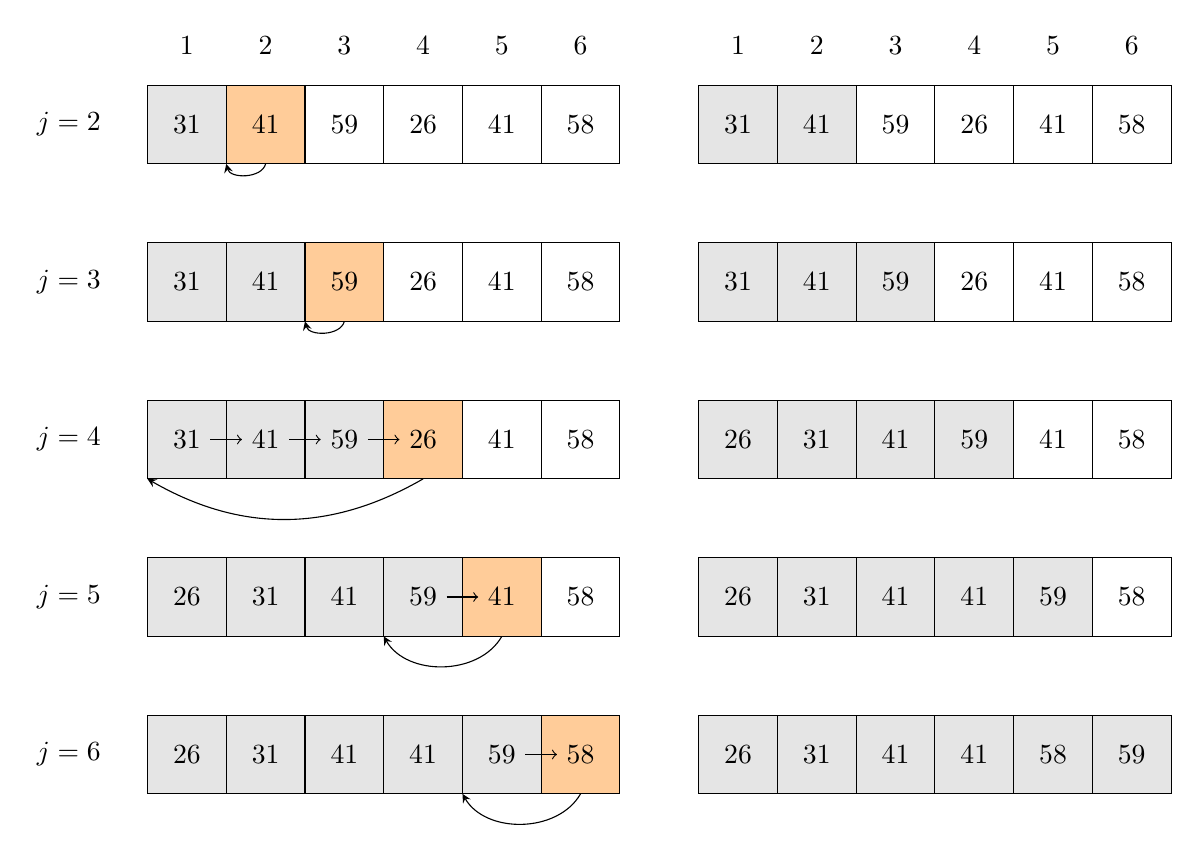
\begin{tikzpicture}
                  %绘制数组上方的索引1,2,3,4,5,6
                  \foreach \i in {1,2,...,6}{\draw (\i,0)+(-.5,+1.5) node {\i};}
                  \foreach \i in {1,2,...,6}{\draw (\i,0)+(6.5,+1.5) node {\i};}
                  %j=2
                  \node (j_2) at (-1,+.5) {$j=2$};
                  %绘制数组矩形
                  \draw[fill=black!10] (0,0) rectangle (1,1);
                  \draw[fill=orange!40] (1,0) rectangle (2,1);
                  \draw (2,0) rectangle (3,1);
                  \draw (3,0) rectangle (4,1);
                  \draw (4,0) rectangle (5,1);
                  \draw (5,0) rectangle (6,1);

                  \draw[fill=black!10] (7,0) rectangle (8,1);
                  \draw[fill=black!10] (8,0) rectangle (9,1);
                  \draw (9,0) rectangle (10,1);
                  \draw (10,0) rectangle (11,1);
                  \draw (11,0) rectangle (12,1);
                  \draw (12,0) rectangle (13,1);
                  %绘制数组中每个元素值
                  \node (A) at (0.5, 0.5) {31};
                  \node (B) at (1.5, 0.5) {41};
                  \node (C) at (2.5, 0.5) {59};
                  \node (D) at (3.5, 0.5) {26};
                  \node (E) at (4.5, 0.5) {41};
                  \node (F) at (5.5, 0.5) {58};

                  \node (A_) at (7.5, 0.5) {31};
                  \node (B_) at (8.5, 0.5) {41};
                  \node (C_) at (9.5, 0.5) {59};
                  \node (D_) at (10.5, 0.5) {26};
                  \node (E_) at (11.5, 0.5) {41};
                  \node (F_) at (12.5, 0.5) {58};
                  %绘制箭头
                  \draw [-stealth] (1.5,0) to[bend left=75] (1,0);

                  %j=3
                  \node (j_3) at (-1,-1.5) {$j=3$};
                  %绘制数组矩形
                  \draw[fill=black!10] (0,-2) rectangle (1,-1);
                  \draw[fill=black!10] (1,-2) rectangle (2,-1);
                  \draw[fill=orange!40] (2,-2) rectangle (3,-1);
                  \draw (3,-2) rectangle (4,-1);
                  \draw (4,-2) rectangle (5,-1);
                  \draw (5,-2) rectangle (6,-1);

                  \draw[fill=black!10] (7,-2) rectangle (8,-1);
                  \draw[fill=black!10] (8,-2) rectangle (9,-1);
                  \draw[fill=black!10] (9,-2) rectangle (10,-1);
                  \draw (10,-2) rectangle (11,-1);
                  \draw (11,-2) rectangle (12,-1);
                  \draw (12,-2) rectangle (13,-1);
                  %绘制数组中每个元素值
                  \node (A) at (0.5, -1.5) {31};
                  \node (B) at (1.5, -1.5) {41};
                  \node (C) at (2.5, -1.5) {59};
                  \node (D) at (3.5, -1.5) {26};
                  \node (E) at (4.5, -1.5) {41};
                  \node (F) at (5.5, -1.5) {58};

                  \node (A_) at (7.5, -1.5) {31};
                  \node (B_) at (8.5, -1.5) {41};
                  \node (C_) at (9.5, -1.5) {59};
                  \node (D_) at (10.5, -1.5) {26};
                  \node (E_) at (11.5, -1.5) {41};
                  \node (F_) at (12.5, -1.5) {58};
                  %绘制箭头
                  \draw [-stealth] (2.5,-2) to[bend left=75] (2,-2);

                  %j=4
                  \node (j_4) at (-1,-3.5) {$j=4$};
                  %绘制数组矩形
                  \draw[fill=black!10] (0,-4) rectangle (1,-3);
                  \draw[fill=black!10] (1,-4) rectangle (2,-3);
                  \draw[fill=black!10] (2,-4) rectangle (3,-3);
                  \draw[fill=orange!40] (3,-4) rectangle (4,-3);
                  \draw (4,-4) rectangle (5,-3);
                  \draw (5,-4) rectangle (6,-3);

                  \draw[fill=black!10] (7,-4) rectangle (8,-3);
                  \draw[fill=black!10] (8,-4) rectangle (9,-3);
                  \draw[fill=black!10] (9,-4) rectangle (10,-3);
                  \draw[fill=black!10] (10,-4) rectangle (11,-3);
                  \draw (11,-4) rectangle (12,-3);
                  \draw (12,-4) rectangle (13,-3);
                  %绘制数组中每个元素值
                  \node (A) at (0.5, -3.5) {31};
                  \node (B) at (1.5, -3.5) {41};
                  \node (C) at (2.5, -3.5) {59};
                  \node (D) at (3.5, -3.5) {26};
                  \node (E) at (4.5, -3.5) {41};
                  \node (F) at (5.5, -3.5) {58};

                  \node (A_) at (7.5, -3.5) {26};
                  \node (B_) at (8.5, -3.5) {31};
                  \node (C_) at (9.5, -3.5) {41};
                  \node (D_) at (10.5, -3.5) {59};
                  \node (E_) at (11.5, -3.5) {41};
                  \node (F_) at (12.5, -3.5) {58};
                  %绘制箭头
                  \draw [-stealth] (3.5,-4) to[bend left=30] (0,-4);
                  \draw [->] (C.east) -- (D.west);
                  \draw [->] (B.east) -- (C.west);
                  \draw [->] (A.east) -- (B.west);

                  %j=5
                  \node (j_5) at (-1,-5.5) {$j=5$};
                  %绘制数组矩形
                  \draw[fill=black!10] (0,-6) rectangle (1,-5);
                  \draw[fill=black!10] (1,-6) rectangle (2,-5);
                  \draw[fill=black!10] (2,-6) rectangle (3,-5);
                  \draw[fill=black!10] (3,-6) rectangle (4,-5);
                  \draw[fill=orange!40] (4,-6) rectangle (5,-5);
                  \draw (5,-6) rectangle (6,-5);

                  \draw[fill=black!10] (7,-6) rectangle (8,-5);
                  \draw[fill=black!10] (8,-6) rectangle (9,-5);
                  \draw[fill=black!10] (9,-6) rectangle (10,-5);
                  \draw[fill=black!10] (10,-6) rectangle (11,-5);
                  \draw[fill=black!10] (11,-6) rectangle (12,-5);
                  \draw (12,-6) rectangle (13,-5);
                  %绘制数组中每个元素值
                  \node (A) at (0.5, -5.5) {26};
                  \node (B) at (1.5, -5.5) {31};
                  \node (C) at (2.5, -5.5) {41};
                  \node (D) at (3.5, -5.5) {59};
                  \node (E) at (4.5, -5.5) {41};
                  \node (F) at (5.5, -5.5) {58};

                  \node (A_) at (7.5, -5.5) {26};
                  \node (B_) at (8.5, -5.5) {31};
                  \node (C_) at (9.5, -5.5) {41};
                  \node (D_) at (10.5, -5.5) {41};
                  \node (E_) at (11.5, -5.5) {59};
                  \node (F_) at (12.5, -5.5) {58};
                  %绘制箭头
                  \draw [-stealth] (4.5,-6) to[bend left=60] (3,-6);
                  \draw [->] (D.east) -- (E.west);

                  %j=6
                  \node (j_6) at (-1,-7.5) {$j=6$};
                  %绘制数组矩形
                  \draw[fill=black!10] (0,-8) rectangle (1,-7);
                  \draw[fill=black!10] (1,-8) rectangle (2,-7);
                  \draw[fill=black!10] (2,-8) rectangle (3,-7);
                  \draw[fill=black!10] (3,-8) rectangle (4,-7);
                  \draw[fill=black!10] (4,-8) rectangle (5,-7);
                  \draw[fill=orange!40] (5,-8) rectangle (6,-7);

                  \draw[fill=black!10] (7,-8) rectangle (8,-7);
                  \draw[fill=black!10] (8,-8) rectangle (9,-7);
                  \draw[fill=black!10] (9,-8) rectangle (10,-7);
                  \draw[fill=black!10] (10,-8) rectangle (11,-7);
                  \draw[fill=black!10] (11,-8) rectangle (12,-7);
                  \draw[fill=black!10] (12,-8) rectangle (13,-7);
                  %绘制数组中每个元素值
                  \node (A) at (0.5, -7.5) {26};
                  \node (B) at (1.5, -7.5) {31};
                  \node (C) at (2.5, -7.5) {41};
                  \node (D) at (3.5, -7.5) {41};
                  \node (E) at (4.5, -7.5) {59};
                  \node (F) at (5.5, -7.5) {58};

                  \node (A_) at (7.5, -7.5) {26};
                  \node (B_) at (8.5, -7.5) {31};
                  \node (C_) at (9.5, -7.5) {41};
                  \node (D_) at (10.5, -7.5) {41};
                  \node (E_) at (11.5, -7.5) {58};
                  \node (F_) at (12.5, -7.5) {59};
                  %绘制箭头
                  \draw [-stealth] (5.5,-8) to[bend left=60] (4,-8);
                  \draw [->] (E.east) -- (F.west);
              \end{tikzpicture}
              \caption{数组$A=[31,41,59,26,41,58]$的插入排序执行过程}\label{练习221}
          \end{figure}
          }
    \item {
          重写过程INSERTION-SORT, 使之按非升序(而不是非降序)排列.\\
          解答: \\
          非升序版本的伪代码如下:
          \begin{codebox}
              \Procname{$\proc{Insertion-Sort}(A)$}
              \li \For $j \gets 2$ \To $\attrib{A}{length}$
              \li \Do
              $\id{key} \gets A[j]$
              \li \Comment Insert $A[j]$ into the sorted sequence
              $A[1 \twodots j-1]$.
              \li $i \gets j-1$
              \li \While $i > 0$ and $A[i] < \id{key}$ \RComment The main difference is here
              \li \Do
              $A[i+1] \gets A[i]$
              \li $i \gets i-1$
              \End
              \li $A[i+1] \gets \id{key}$
              \End
          \end{codebox}
          非升序版本和非降序版本的主要差别在于将$A[j]$插入已排序的序列$A[1 \twodots j-1]$这一步. 非升序版本的Python实现为:
          \lstinputlisting[style=Python]{./codes/exercise_2_1_2.py}
          }
    \item {
          考虑以下\textbf{查找问题}:\\
          \textbf{输入: }$n$个数的一个序列$A=\langle a_{1},a_{2},\dots,a_{n} \rangle$和一个值$v$.\\
          \textbf{输出: }下标$i$使得$v=A[i]$或者当$v$不在$A$中出现时, $v$为特殊值NIL.\\
          写出\textbf{线性查找}的伪代码, 它扫描整个序列来查找$v$. 使用一个循环不变式来证明你的算法是正确的. 确保你的循环不变式满足三条必要的性质.\\
          解答: \\
          线性查找的算法描述为:
          \begin{codebox}
              \Procname{$\proc{Linear-Search}(A,v)$}
              \li \For $i \gets 1$ \To $\attrib{A}{length}$
              \li     \Do
              \If $A[i] \isequal v$
              \li         \Then \Return $i$
              \End
              \End
              \li \Return \const{NIL}
          \end{codebox}

          其Python实现为:

          \lstinputlisting[style=Python]{./codes/exercise_2_1_3.py}

          循环不变式的证明如下:

          \textbf{初始化: }在循环迭代开始之前, 相当于没有遍历过任何元素, 自然不可能找到目标元素$v$, 所以函数不会return, 循环必定可以开始.

          \textbf{保持: }若循环能进行下去, 则意味着在子数组$A[1..i-1]$内没有找到目标元素$v$, 因此需要考察第$i$个元素. 在考察完第$i$个元素之后, “在子数组$A[1..i-1]$内没有找到目标元素$v$”这一命题仍然为真.

          \textbf{终止: }一种情况是, 当考察到第$i$个元素时, 若$A[i]$等于$v$, 则意味着已经找到目标元素, 直接返回$i$. 另一种情况是, 循环迭代的终止是由于$i$大于数组$A$的长度$n$, 此时$i=n+1$. 那么根据前两条性质可知, 子数组$A[1..i-1]$内没有找到目标元素$v$. 此时的子数组恰好是原问题数组, 意味着数组$A$内不存在目标元素$v$, 故返回NIL.
          }
    \item {
          考虑把两个$n$位二进制整数加起来的问题, 这两个整数分别存储在两个$n$元数组$A$和$B$中. 这两个整数的和应按二进制形式存储在一个$(n+1)$元数组$C$中. 请给出该问题的形式化描述, 并写出伪代码.\\
          解答: \\
          算法描述为:
          \begin{codebox}
              \Procname{$\proc{Add-Binary}(A,B)$}
              \li $int[n+1] \id{C} \gets \{0,\twodots,0\}$ \RComment $n=\attrib{A}{length}$
              \li $\id{val} \gets 0$ \RComment 用于保存下一位(进位)值的变量
              \li \For $i \gets n \To 1$
              \li     \Do
              $\id{sum} = A[i]+B[i]+\id{val}$
              \li     \If $\id{sum} \isequal 3$ \Then \RComment 当前位求和为3
              \li         $\id{val} \gets 1$ \RComment 进位1
              \li         $C[i+1] \gets 1$ \RComment 当前位余1
              \li     \ElseIf $\id{sum} \isequal 2$ \Then \RComment 当前位求和为2
              \li         $\id{val} \gets 1$ \RComment 进位1
              \li         $C[i+1] \gets 0$ \RComment 当前位余0
              \li     \Else
              \li         $\id{val} \gets 0$ \RComment 不进位
              \li         $C[i+1] \gets \id{sum}$ \RComment 当前位余$\id{sum}$
              \End
              \End
              \li $C[1] \gets \id{val}$
              \li \Return $\id{C}$
          \end{codebox}
          }
\end{enumerate}

%第2节
\section{分析算法}

\subsection*{最坏情况与平均情况分析}

对于插入排序, 最好情况下, $T(n)=an+b$, 最坏情况下, $T(n)=an^2+bn+c$.

我们往往集中于只求\textbf{最坏情况运行时间}, 即对规模为$n$的任何输入, 算法的最长运行时间, 这样做的三点理由:
\begin{itemize}
    \item 一个算法的最坏情况运行时间给出了任何输入的运行时间的一个上界. 知道了这个界, 就能确保该算法绝不需要更长的时间. 我们不必对运行时间做某种复杂的猜测并可以期望它不会变得更坏.
    \item 对某些算法, 最坏情况经常出现. 例如, 当在数据库中检索一条特定的信息时, 若该信息不在数据库中出现, 则检索算法的最坏情况会经常出现. 在某些应用中, 对缺失信息的检索可能是频繁的.
    \item “平均情况”往往与最坏的情况大致一样差. 假定随机选择$n$个数并应用插入排序. 需要多长时间来确定在子数组$A[1..j-1]$的什么位置插入元素$A[j]$? 平坤来说, $A[1..j-1]$中的一半元素小于$A[j]$, 一半元素大于$A[j]$. 所以, 平均来说, 我们检查子数组$A[1..j-1]$的一半, 那么$t_{j}$大约为$j/2$. 导致的平均情况运行时间结果像最坏情况运行时间一样, 也是输入规模的一个二次函数.
\end{itemize}

在某些特定的情况下, 我们会对一个算法的\textbf{平均情况}运行时间感兴趣; 贯穿于本书, 我们将看到\textbf{概率分析}技术被用于各种算法. 平均情况分析的范围有限, 因为对于特定的问题, 什么构成一种“平均”输入并不明显. 我们常常假定给定规模的所有输入具有相同的可能性. 实际上, 该假设可能不成立, 但是, 有时可以使用\textbf{随机化算法}, 它做出一些随机的选择, 以允许进行概率分析并产生某个\textbf{期望}的运行时间. 在第5章以及后续的其它几章中, 我们将进一步探究随机化算法.

\subsection*{增长量级}

我们真正感兴趣的是运行时间的\textbf{增长率}或\textbf{增长量级}. 一般会忽略低阶项, 保留高阶项. 以插入排序为例, 记最坏情况的运行时间$\Theta(n^2)$(读作“theta n平方”).

\subsection*{练习}
\begin{enumerate}
    \renewcommand{\labelenumi}{\thesection-\theenumi}
    \item {用$\Theta$记号表示函数$n^3/1000-100n^2-100n+3$.\\
          解答: $\Theta(n^3)$}
    \item {考虑排序存储在数组A中的$n$个数: 首先找出A中的最小元素并将其与$A[1]$中的元素进行交换. 接着, 找出$A$中的次最小元素并将其与$A[2]$中的元素进行交换. 对$A$中前$n-1$个元素按该方式继续. 该算法称为\textbf{选择算法}, 写出其伪代码. 该算法维持的循环不变式是什么? 为什么它只需要对前$n-1$个元素, 而不是对所有$n$个元素运行? 用$\Theta$记号给出选择排序的最好情况与最坏情况的运行时间.\\
          解答: \\
          选择算法的伪代码为:
          \begin{codebox}
              \Procname{$\proc{Selection-Sort}(A)$}
              \li \For $i \gets 1$ \To $\attrib{A}{length} - 1$ \Do
              \li     $\id{minIndex} \gets i$
              \li     \For $j \gets i + 1$ \To $\attrib{A}{length}$ \Do
              \li         \If $A[j] \le A[minIndex]$ \Then
              \li             $\id{minIndex} \gets j$
              \End
              \End
              \li     $\id{temp} \gets A[i]$
              \li     $A[i] \gets A[minIndex]$
              \li     $A[minIndex] \gets temp$
              \End
          \end{codebox}
          }
\end{enumerate}

%第3节
\section{设计算法}
\subsection{分治法}

\subsection{分析分治算法}

%%%%%分割线%%%



\end{document}
